% !TEX root = ../slides.tex

\begin{frame}[label=spectral_properties_2]
\frametitle{Spectral point of view (2/2)}

\centering
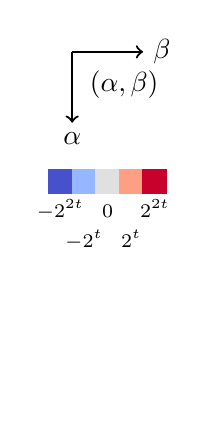
\begin{tikzpicture}[scale=.3]
\draw[->,thick] (0,0)--(3,0) node[right]{$\beta$};
\draw[->,thick] (0,0)--(0,-3) node[below]{$\alpha$};
\node at (2.2, -1.4) { $\cFh(\alpha, \beta)$};
\draw[transparent] (0, -15) rectangle (1, 1) ;

\definecolor{orangeLAT}{HTML}{fe9e82}
\definecolor{redLAT}{HTML}{c7002c}
\definecolor{lightblueLAT}{HTML}{96b6ff}
\definecolor{blueLAT}{HTML}{4851cc}
\definecolor{greyLAT}{HTML}{e1e0e0}


\draw[blueLAT, fill=blueLAT] (-1, -6) rectangle node[below=3] {\scriptsize \color{black} ${-2}^{2t}$} (0, -5);
\draw[lightblueLAT, fill=lightblueLAT] (0, -6) rectangle node[below=14] {\scriptsize \color{black} ${-2}^t$} (1, -5);
\draw[greyLAT, fill=greyLAT] (1, -6) rectangle node[below=5] {\scriptsize \color{black} $0$} (2, -5);
\draw[orangeLAT, fill=orangeLAT] (2, -6) rectangle node[below=14] {\scriptsize \color{black} $2^t$} (3, -5);
\draw[redLAT, fill=redLAT] (3, -6) rectangle node[below=3] {\scriptsize \color{black} $2^{2t}$} (4, -5);

\end{tikzpicture}
\begin{overpic}[scale=.1]{figures/kim_lat}
          \begin{tikzpicture}[scale=6.5]
            \draw[transparent] (0, 0) rectangle (1, 1) ;
            % \onslide<2>{
            %   \draw[ForestGreen, line width=.8mm] (0.17, 0.69) circle (2pt);
            %   \draw[ForestGreen, line width=.8mm] (0.17, 0.16) circle (2pt);
            %   \draw[ForestGreen, line width=.8mm] (0.81, 0.89) circle (2pt);
            %   \draw[ForestGreen, line width=.8mm] (0.81, 0.38) circle (2pt);
            %   }
            \onslide<2>{
              \draw[yellow, line width=.8mm] (0, 0.94) rectangle (.98, .99);
            }
          \end{tikzpicture}
        \end{overpic}
\includegraphics[scale=.1]{figures/cube_lat}

\begin{textblock*}{10cm}(.8cm,8.5cm)
Kim mapping $\kim \from \clambda \mapsto \clambda^3 + \clambda^{10} + u\clambda^{24}$
\end{textblock*}

\begin{textblock*}{5cm}(9.5cm,8.5cm)
Cube over $\FF_{64}$ $\clambda \mapsto \clambda^3$
\end{textblock*}


\end{frame}